\documentclass[tikz,border=4pt]{standalone}
\usepackage{ctex}
\usepackage{amsmath}
\usepackage{pgfplots}
\pgfplotsset{compat=1.18}
\begin{document}
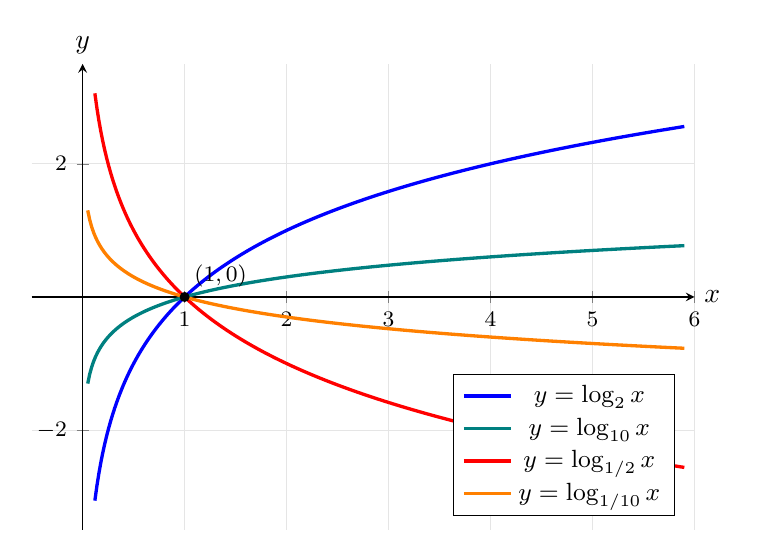
\begin{tikzpicture}
\begin{axis}[
    axis lines=middle,
    xmin=-0.5, xmax=6.0,
    ymin=-3.5, ymax=3.5,
    width=10cm, height=7.5cm,
    xlabel={$x$}, ylabel={$y$},
    xlabel style={right}, ylabel style={above},
    samples=300,
    grid=both,
    grid style={gray!20},
    legend pos=south east,
    legend style={font=\small},
    tick label style={font=\footnotesize},
]
\addplot[blue, very thick, domain=0.12:5.9] {ln(x)/ln(2)};
\addlegendentry{$y=\log_2 x$}
\addplot[teal, very thick, domain=0.05:5.9] {ln(x)/ln(10)};
\addlegendentry{$y=\log_{10} x$}
\addplot[red, very thick, domain=0.12:5.9] {ln(x)/ln(1/2)};
\addlegendentry{$y=\log_{1/2} x$}
\addplot[orange, very thick, domain=0.05:5.9] {ln(x)/ln(1/10)};
\addlegendentry{$y=\log_{1/10} x$}
\addplot[only marks, mark=*, mark size=1.6pt, black] coordinates {(1,0)};
\node[above right, font=\footnotesize] at (axis cs:1,0) {$(1,0)$};
\end{axis}
\end{tikzpicture}
\end{document}
